\documentclass{standalone}
\usepackage[usenames,dvipsnames]{xcolor}
\usepackage{amsmath, amssymb, amsthm}

\usepackage{tikz}
\begin{document}
	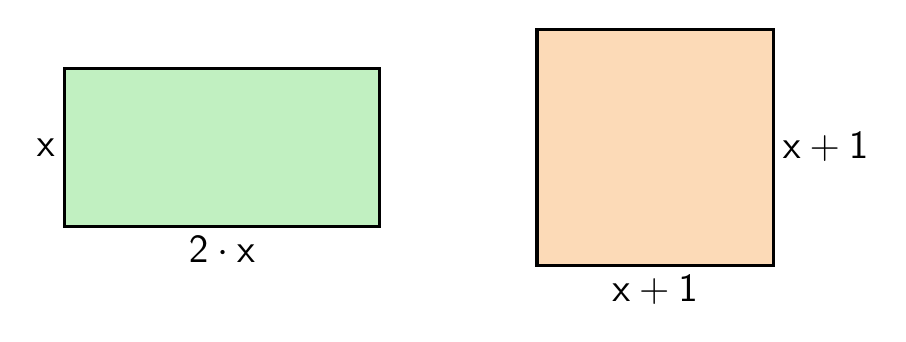
\begin{tikzpicture}[font=\small]
		\draw[black, very thick, fill=LimeGreen, fill opacity=0.3] (0,0) rectangle (4,2);
		\draw[black] (0,1) node [left] {\Large $\mathsf{x}$};
		\draw[black] (2,0) node [below] {\Large $\mathsf{2\cdot x}$};
		\draw[black, very thick, fill=BurntOrange, fill opacity=0.3] (6,-0.5) rectangle ++ (3,3);
		\draw[black] (7.5,-0.5) node [below] {\Large $\mathsf{x+1}$};
		\draw[black] (9,1) node [right] {\Large $\mathsf{x+1}$};
	\end{tikzpicture}
\end{document}